\begin{frame}{Experimental Results}
	\begin{minipage}{0.54\textwidth}
	\begin{itemize}
	\item Daubechies filter used for DWT
	\item three-level pyramid decomposition
	\item watermark embedding in high resolution subbands $LH_3$, $HL_3$, $HH_3$ 
	\item embedding strength $\alpha$ constant \\ $\rightarrow$ chosen that PSNR = 45dB
	\item each subband $B$ has $N_B$ = 4096 coefficients% \\$\rightarrow$ $N = 3 \times N_B = 12288$
	\end{itemize}
	\end{minipage} 
	\begin{minipage}{0.44\textwidth}
	\begin{figure}
	\centering
	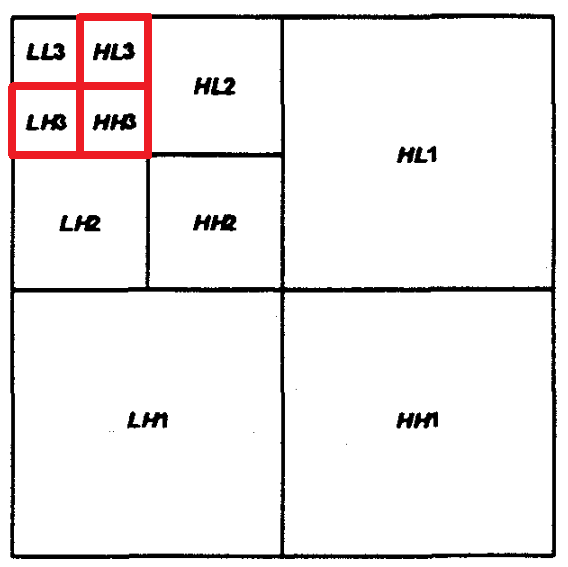
\includegraphics[width=\textwidth]{Bilder/threelayerMotivationPainted} 
	\end{figure}
	\end{minipage} 	
\end{frame}

\begin{frame}{Experimental Results}
	\begin{minipage}{0.54\textwidth}
	\begin{itemize}
	\item blind detection is used
	\item estimation of $\mu_i$ and $\sigma_i$ from watermarked image:
	\end{itemize}
$$\hat{\mu}_i = \frac{1}{N_B} \sum_{y \in B}y$$
	$$\hat{\sigma}_i = \frac{1}{N_B - 1} \sum_{y\in B}(y-\hat{\mu}_i)^2$$ 
	\end{minipage} 
	\begin{minipage}{0.44\textwidth}
	\begin{figure}
	\centering
	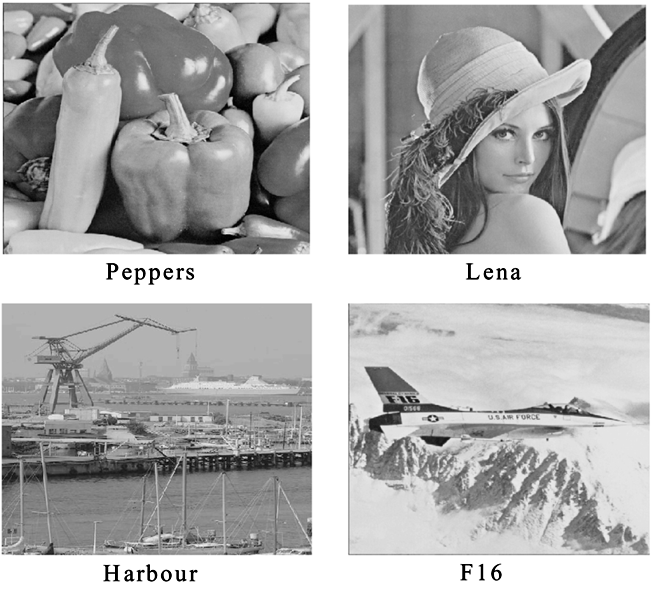
\includegraphics[width=\textwidth]{Bilder/ResultsBilder} 
	\end{figure}
	\end{minipage} 	
	with $y$ as DWT coefficient in $B$ of watermarked image
\end{frame}